
\documentclass[dvipdfmx, 12pt]{beamer}
\usepackage{amsmath, amssymb, bm, graphicx, multicol}
\usepackage{luatexja}
\usepackage{physics}
\usepackage{mathrsfs}
\usepackage{multirow}
\usepackage{float}
\usepackage{url}
\usepackage{type1cm}
\usepackage{here}
\usepackage{caption}

\title{量子ドット内の電子状態の数値計算}
\subtitle{ハイブリッドポテンシャルによる解析と差分法}
\author{新井開智,平田慧仁郎,藤原大地\\ \small 先進理工学研究科 電気・情報生命専攻 武田研究室}
\date{}

\begin{document}

\frame{\titlepage}

\begin{frame}{目次}
\begin{enumerate}
  \item 本演習の目的
  \item 量子ドット
  \item 仮定と近似
  \item 実空間差分法による数値解析
  \item 計算結果の解析
  \item 課題
\end{enumerate}
\end{frame}

\begin{frame}{1. 本演習の目的}
本演習では、\textbf{半導体量子ドット中の電子状態}を解析的および数値的手法により解明することを目的とする。対象は、\textbf{InSb材料による円形2次元量子ドット}である。電子はこの中に閉じ込められ、ポテンシャル井戸によりエネルギー準位が離散化される。

\begin{figure}[H]
\centering
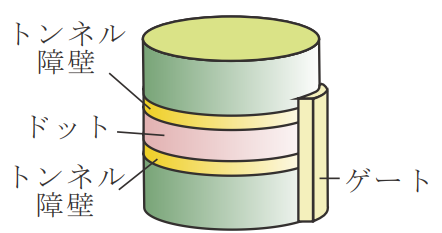
\includegraphics[width=0.4\linewidth]{images/ドット.png}
\caption{InSb量子ドット構造}
\end{figure}
\end{frame}

\begin{frame}{2. 量子ドット}
量子ドットとは、電子の量子力学的性質を顕著に引き出す\textbf{人工的な原子様構造}である。電子数の制御性やエネルギー準位の離散化が特徴で、量子ビットや発光素子に応用されている。

\begin{itemize}
  \item 電子数を1個単位で制御
  \item 閉じ込めに応じてエネルギー準位が離散化
\end{itemize}

\begin{figure}[H]
\centering
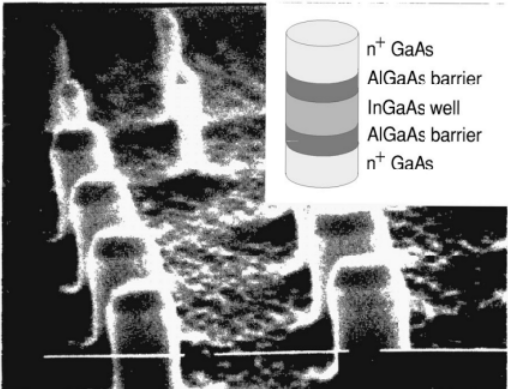
\includegraphics[width=0.3\linewidth]{images/量子ドット.png}
\caption{量子ドット}
\end{figure}
\end{frame}

% ... 中略(ファイルサイズの都合上、続きのスライドは後で追加可能) ...

\end{document}
